\section{Framework}

We define educational AI tasks along two axes. The first axis is \emph{knowledge-grounding need}: the extent to which success depends on retrieving accurate, task-relevant evidence from an external corpus or tool. The second axis is \emph{pedagogical coordination complexity}: the extent to which success depends on decomposition, adaptive sequencing, feedback refinement, critique, learner modeling, or role-specialized reasoning. The value of the framework is not that it predicts winners with certainty, but that it forces architectural comparisons to state which difficulty is actually being tested.

Under this framing, classical RAG should remain strong in the high-grounding, low-coordination regime. Examples include evidence-grounded question answering over course materials, reference-backed short explanations, and citation-sensitive factual support. As pedagogical coordination complexity rises, however, retrieval may remain necessary without remaining sufficient. Tasks such as adaptive tutoring, rubric-based critique, and study-plan generation require the system to decide \emph{how} to teach, not merely \emph{what} evidence to surface. Agentic RAG and non-RAG multi-agent systems represent two different ways to handle that transition: the former keeps retrieval central while adding orchestration, whereas the latter tests whether specialized coordination can dominate when evidence need is lower.

\subsection{Architectural families}

The paper keeps four comparison families distinct.

\begin{itemize}[leftmargin=*]
    \item \textbf{Classical RAG:} a single retrieve-then-generate pipeline with fixed retrieval access and no explicit planning or critique loop.
    \item \textbf{Agentic RAG:} retrieval remains available, but planning, critique, rerouting, or tool use can shape how evidence is gathered and applied.
    \item \textbf{Non-RAG multi-agent systems:} multiple specialized agents coordinate without treating retrieval as the default controller.
    \item \textbf{Single-agent no-RAG baseline:} a control condition that helps separate retrieval gains and coordination gains from general model quality.
\end{itemize}

This separation matters because many papers collapse materially different systems into a generic ``agentic'' category. Our argument depends on keeping them separate. A planner wrapped around retrieval is not the same architectural claim as a tutoring stack built from diagnoser, rubric, tutor, and critic agents with retrieval invoked only when the task clearly requires external evidence.

\subsection{Task taxonomy}

Table~\ref{tab:task-taxonomy} summarizes the working taxonomy used throughout the paper. The labels are hypotheses to be tested rather than declared winners.

\begin{table}[t]
\centering
\small
\begingroup
\setlength{\tabcolsep}{4pt}
\begin{tabular}{@{}>{\raggedright\arraybackslash}p{0.26\linewidth}>{\raggedright\arraybackslash}p{0.2\linewidth}>{\raggedright\arraybackslash}p{0.2\linewidth}>{\raggedright\arraybackslash}p{0.3\linewidth}@{}}
\toprule
Task regime & Grounding need & \shortstack[c]{Coordination\\complexity} & \shortstack[c]{Hypothesized strong\\architecture} \\
\midrule
Evidence-grounded educational QA & High & Low & Classical RAG \\
Source-grounded explanation & High & Low to medium & Classical or agentic RAG \\
Rubric-based feedback & Medium & Medium to high & Agentic RAG or multi-agent orchestration \\
Adaptive tutoring dialogue & Low to medium & High & Multi-agent orchestration or agentic RAG \\
Lesson or study planning & Low to medium & High & Multi-agent orchestration \\
\bottomrule
\end{tabular}
\endgroup
\caption{Working task taxonomy for comparing retrieval-centric and coordination-centric educational AI architectures. The labels identify hypotheses to be stress-tested against benchmark evidence rather than completed findings.}
\label{tab:task-taxonomy}
\end{table}

The taxonomy is useful because it makes negative results interpretable. If classical RAG remains best on simple evidence-grounded tasks, that is not a failure of the framework; it is evidence that retrieval remains the right abstraction there. If non-RAG multi-agent systems fail on citation-sensitive tasks, that likewise strengthens the taxonomy by showing where orchestration alone is insufficient.

\subsection{A repository-grounded tutoring instantiation}

The article is also grounded in a concrete tutoring implementation already present in the repository. The \texttt{ConferenceEduSystem} codebase exposes executable families corresponding to classical RAG, hybrid-fast agentic RAG, non-RAG multi-agent tutoring, and single-agent no-RAG. Rather than assuming one family should dominate globally, the system uses a lightweight regime router that treats retrieval as conditional.

Figure~\ref{fig:arch} summarizes the design. A common educational input first reaches a routing stage. Classical RAG follows a direct retriever-to-tutor path. The hybrid-fast path runs planner, diagnoser, and rubric agents in parallel, invokes retrieval only when evidence need is high, then passes through tutor and critic stages. The non-RAG path emphasizes planner, diagnoser, rubric, tutor, and critic coordination without retrieval as the default controller. Two side components are especially relevant to the educational claim: a student-state tracker that collects learner level, confusion cues, misconceptions, and explanation style; and a retrieval subsystem built from a hybrid index plus lightweight reranking.

\begin{figure}[t]
\centering
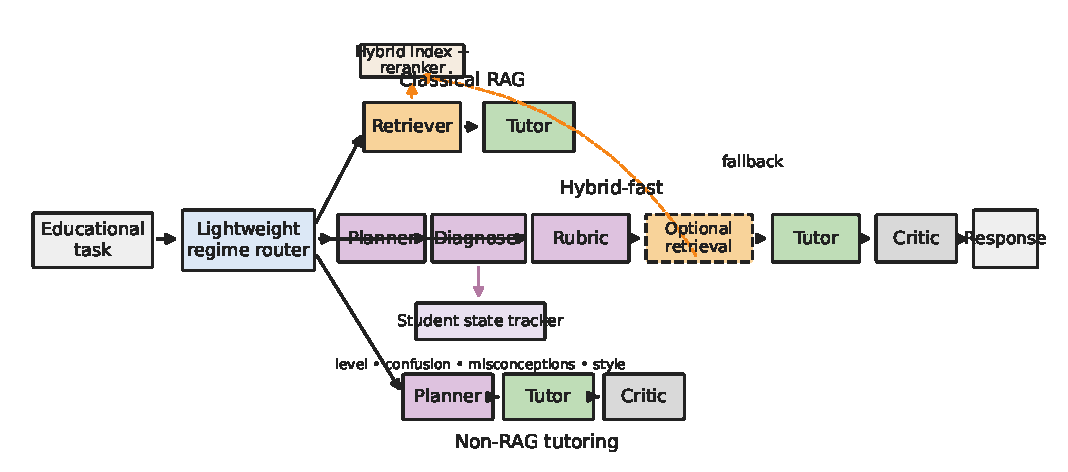
\includegraphics[width=0.9\linewidth]{build-artifacts/adaptive_tutoring_architecture.pdf}
\caption{Repository-grounded adaptive tutoring architecture with a lightweight regime router selecting among classical RAG, hybrid-fast agentic RAG, and non-RAG multi-agent tutoring.}
\label{fig:arch}
\end{figure}

This repository-grounded framing narrows the paper's claims. We are not arguing that every educational system should adopt full multi-agent orchestration. We are arguing that once tutoring quality depends on learner diagnosis, rubric following, critique, and strategy selection, retrieval often becomes one component inside a broader policy rather than the sole organizing principle.

Figure~\ref{fig:loop} makes the same claim at the interaction level. The diagnoser and student-state tracker maintain a serializable account of learner level, confusion cues, misconceptions, and preferred explanation style. Planning and rubric control then decide whether the next tutoring move should be a hint, a worked step, a rubric-grounded critique, or a retrieval-backed explanation. Retrieval remains optional and is triggered only when external evidence is necessary for the pedagogical move.

\begin{figure}[t]
\centering
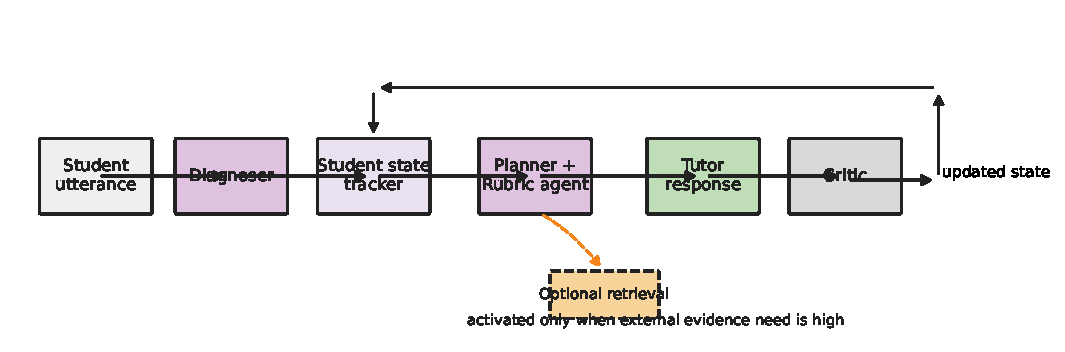
\includegraphics[width=0.95\linewidth]{build-artifacts/student_state_tutoring_loop.pdf}
\caption{Student-state-aware tutoring loop. Retrieval appears as a conditional branch rather than as the default response path.}
\label{fig:loop}
\end{figure}

\subsection{Research questions and hypotheses}

The manuscript is organized around two research questions.

\begin{enumerate}[label=RQ\arabic*:,leftmargin=*]
    \item Under what educational task conditions is classical RAG sufficient, and when do agentic or multi-agent systems become justified?
    \item What evaluation design can compare classical RAG, agentic RAG, and non-RAG multi-agent systems fairly under shared tasks, budgets, and source corpora?
\end{enumerate}

To keep the framing falsifiable, the paper adopts balanced hypotheses rather than a universal superiority claim.

\begin{enumerate}[label=H\arabic*:,leftmargin=*]
    \item On low-coordination, knowledge-grounded educational tasks, classical RAG will perform comparably to or better than more complex multi-agent systems at lower cost.
    \item On coordination-heavy educational tasks such as adaptive tutoring, rubric-based critique, and multi-step study planning, agentic or multi-agent systems may outperform classical RAG on pedagogical quality and adaptivity.
    \item Non-RAG multi-agent systems will underperform retrieval-enabled systems on fact-intensive or citation-sensitive tasks, showing that orchestration alone does not remove the need for grounding.
    \item In mixed regimes, hybrid systems that combine orchestration with conditional retrieval will often define the strongest quality--latency trade-off.
\end{enumerate}
